\documentclass[border=10pt]{standalone}
\usepackage[svgnames]{xcolor}
\usepackage{amsmath}
\usepackage{pgfplots}
\pgfplotsset{compat=newest}
\usepackage[sfdefault]{FiraSans}
\usepackage{FiraMono}
\renewcommand*\familydefault{\sfdefault}
\begin{document}
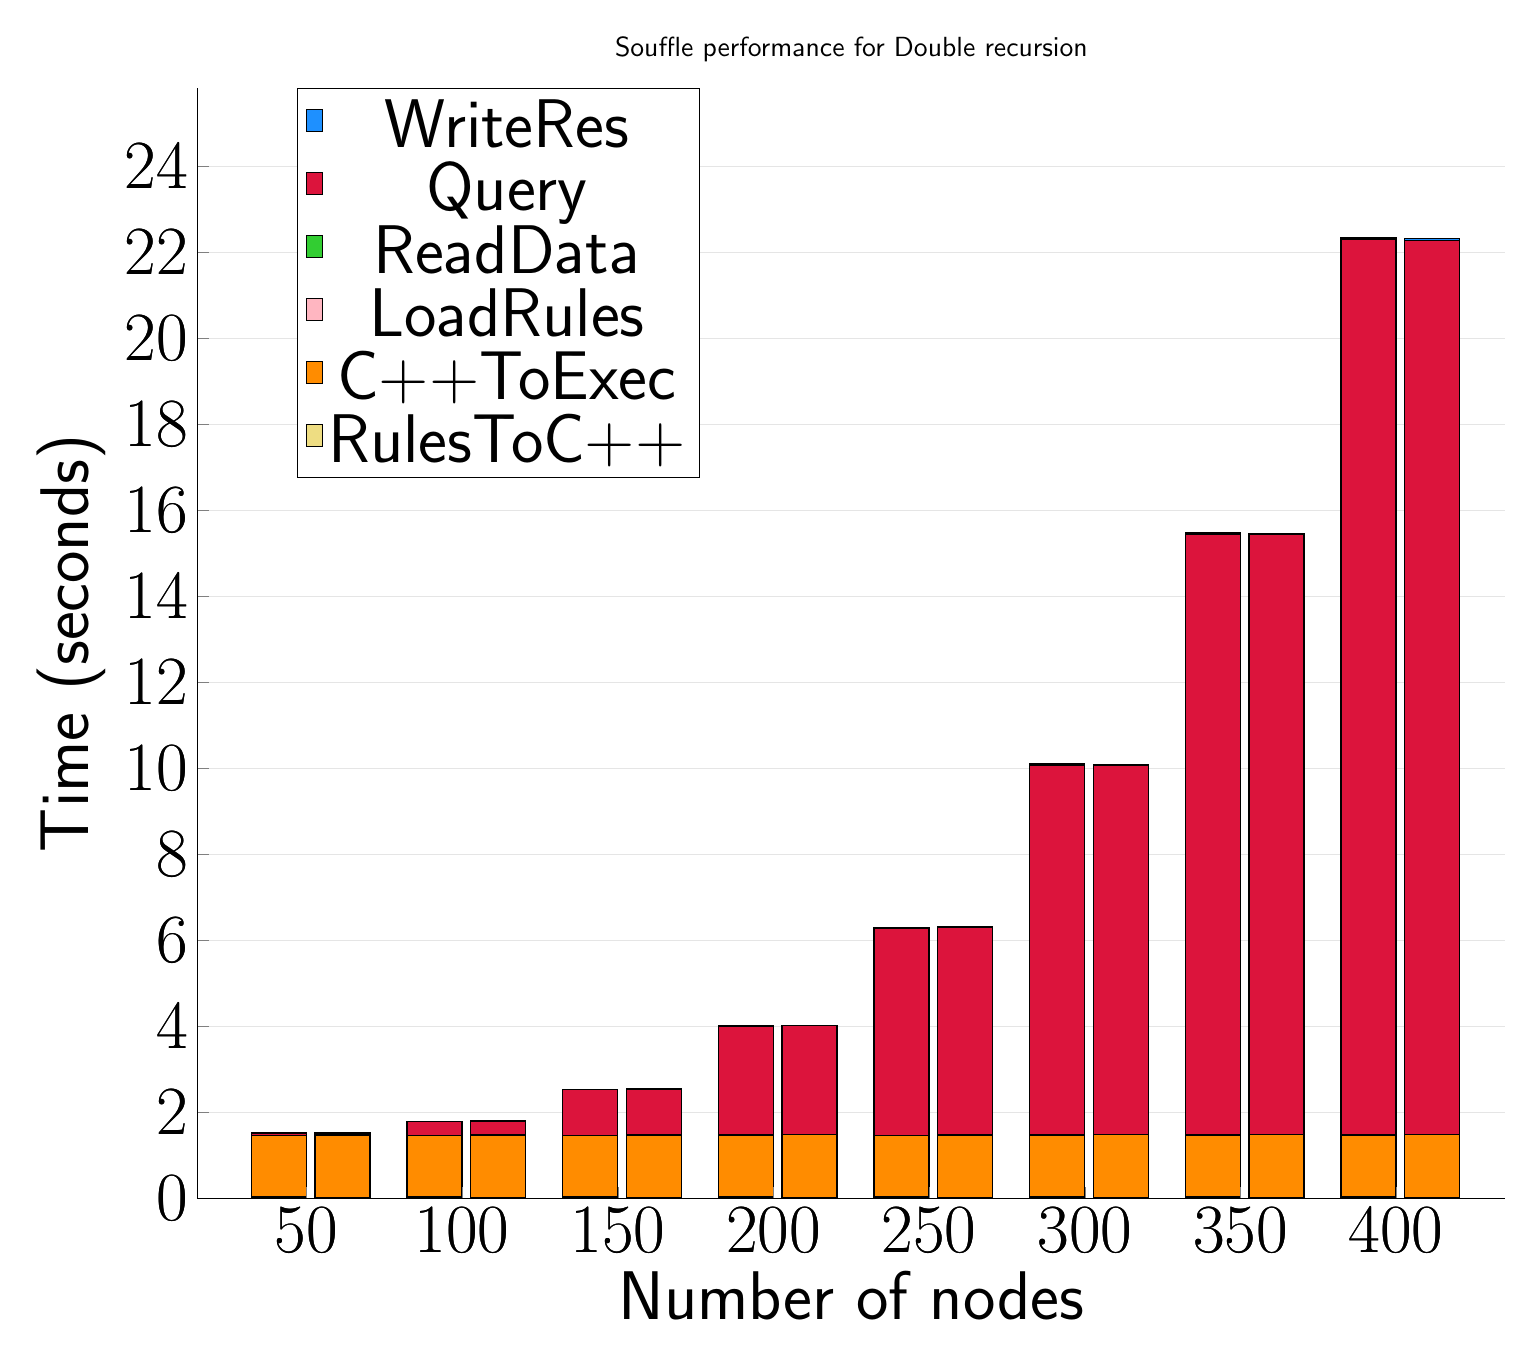
\begin{tikzpicture}
	\begin{axis}[
			ybar stacked,
			title={Souffle performance for Double recursion},
			bar shift=-10pt,
			width=1.5\textwidth,
			bar width=0.7cm,
			ymajorgrids, tick align=inside,
			major grid style={draw=gray!20},
			xtick=data,
			ymin=0, ymax=25.820519999999995,
			axis x line*=bottom,
			axis y line*=left,
			enlarge x limits=0.1,
			legend style={
					at={(0.23, 1)},
					anchor=north,
					legend columns=1,
					font=\Huge,
				},
			ylabel={Time (seconds)},
			xlabel={Number of nodes},
			label style={font=\Huge},
			tick label style={font=\Huge},
		]
		\addlegendimage{fill=DodgerBlue, draw=black, line width=0.2pt}
		\addlegendentry{WriteRes}
		\addlegendimage{fill=Crimson, draw=black, line width=0.2pt}
		\addlegendentry{Query}
		\addlegendimage{fill=LimeGreen, draw=black, line width=0.2pt}
		\addlegendentry{ReadData}
		\addlegendimage{fill=LightPink, draw=black, line width=0.2pt}
		\addlegendentry{LoadRules}
		\addlegendimage{fill=DarkOrange, draw=black, line width=0.2pt}
		\addlegendentry{C++ToExec}
		\addlegendimage{fill=LightGoldenrod, draw=black, line width=0.2pt}
		\addlegendentry{RulesToC++}
		\addplot +[fill=LightGoldenrod, draw=black, line width=0.5pt] coordinates {
				(50, 0.039999961853027344)
				(100, 0.039999985694885255)
				(150, 0.04000003337860107)
				(200, 0.039999985694885255)
				(250, 0.04000000953674317)
				(300, 0.04100017547607422)
				(350, 0.04100000858306885)
				(400, 0.040999960899353025)
			};
		\addplot +[fill=DarkOrange, draw=black, line width=0.5pt] coordinates {
				(50, 1.4259999990463257)
				(100, 1.427999997138977)
				(150, 1.4240000009536744)
				(200, 1.4349999904632569)
				(250, 1.4239999771118164)
				(300, 1.4379998207092286)
				(350, 1.4399999618530273)
				(400, 1.440000057220459)
			};
		\addplot +[fill=LightPink, draw=black, line width=0.5pt] coordinates {
				(50, 0.00011009609999999999)
				(100, 0.0001115876)
				(150, 8.65331e-05)
				(200, 9.992489999999998e-05)
				(250, 0.00012141659999999998)
				(300, 9.695000000000001e-05)
				(350, 0.00011305010000000002)
				(400, 0.0001118624)
			};
		\addplot +[fill=LimeGreen, draw=black, line width=0.5pt] coordinates {
				(50, 0.00036799590000000007)
				(100, 0.0004549625)
				(150, 0.0005579208)
				(200, 0.0006598125999999998)
				(250, 0.0007967458)
				(300, 0.0008591288000000001)
				(350, 0.0009422411000000001)
				(400, 0.0010405165000000002)
			};
		\addplot +[fill=Crimson, draw=black, line width=0.5pt] coordinates {
				(50, 0.05277334)
				(100, 0.3237246)
				(150, 1.068322)
				(200, 2.537682)
				(250, 4.825049000000001)
				(300, 8.599152999999998)
				(350, 13.96757)
				(400, 20.820519999999995)
			};
		\addplot +[fill=DodgerBlue, draw=black, line width=0.5pt] coordinates {
				(50, 0.0009531211999999999)
				(100, 0.003066887)
				(150, 0.006657872999999999)
				(200, 0.011873659999999998)
				(250, 0.01813429)
				(300, 0.025627650000000002)
				(350, 0.03495655)
				(400, 0.04509358)
			};
	\end{axis}
	\begin{axis}[
			ybar stacked,
			bar shift=13pt,
			width=1.5\textwidth,
			bar width=0.7cm,
			ymajorgrids, tick align=inside,
			major grid style={draw=none},
			xtick=data,
			ymin=0, ymax=25.820519999999995,
			axis x line*=none,
			axis y line*=none,
			enlarge x limits=0.1,
			label style={font=\Huge},
			tick label style={font=\Huge},
		]
		\addplot +[fill=LightGoldenrod, draw=black, line width=0.5pt] coordinates {
				(50, 0.030000000000000006)
				(100, 0.030000000000000006)
				(150, 0.030000000000000006)
				(200, 0.030000000000000006)
				(250, 0.030000000000000006)
				(300, 0.030000000000000006)
				(350, 0.030000000000000006)
				(400, 0.030000000000000006)
			};
		\addplot +[fill=DarkOrange, draw=black, line width=0.5pt] coordinates {
				(50, 1.4439999999999997)
				(100, 1.4469999999999996)
				(150, 1.4449999999999998)
				(200, 1.4550000000000003)
				(250, 1.4499999999999997)
				(300, 1.457)
				(350, 1.4600000000000002)
				(400, 1.4580000000000002)
			};
		\addplot +[fill=LightPink, draw=black, line width=0.5pt] coordinates {
				(50, 0.0001075)
				(100, 0.00011080000000000001)
				(150, 8.6e-05)
				(200, 9.94e-05)
				(250, 0.00012030000000000001)
				(300, 9.63e-05)
				(350, 0.00011220000000000002)
				(400, 0.00011099999999999999)
			};
		\addplot +[fill=LimeGreen, draw=black, line width=0.5pt] coordinates {
				(50, 0.0003652)
				(100, 0.00045390000000000003)
				(150, 0.0005567999999999999)
				(200, 0.0006571999999999999)
				(250, 0.0007957999999999999)
				(300, 0.0007892000000000001)
				(350, 0.0008537)
				(400, 0.0009533)
			};
		\addplot +[fill=Crimson, draw=black, line width=0.5pt] coordinates {
				(50, 0.0526721)
				(100, 0.3230982)
				(150, 1.066175)
				(200, 2.532561)
				(250, 4.815493)
				(300, 8.581636)
				(350, 13.94141)
				(400, 20.779619999999998)
			};
		\addplot +[fill=DodgerBlue, draw=black, line width=0.5pt] coordinates {
				(50, 0.0009512000000000001)
				(100, 0.0030570000000000003)
				(150, 0.0064953)
				(200, 0.0115408)
				(250, 0.0179507)
				(300, 0.0255558)
				(350, 0.0347213)
				(400, 0.044857400000000006)
			};
	\end{axis}
\end{tikzpicture}

\end{document}
